\scanpage{49}
\mspage{\handwritten{17}}
\margin{\handwritten{\figure{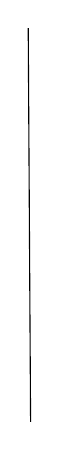
\begin{tikzpicture}\draw (0,0)--(.03,-5);\end{tikzpicture}}}}
\uline{Proposition} 11.\begin{tikzpicture}[x=1cm,y=1cm,baseline=(n.base)]\node (n) at (0,0) {11};\draw (-.15,.3)--(-.02,.3);\draw (-.07,-.08)--(-.07,-.25);\end{tikzpicture}. Soi\deleted{\unsure{ent}}\handwritten{t} \deleted{$k$ un corps}, $G$ un \deleted{schéma en }groupe\deleted{s quasi-compact}\inserted{\handwritten{algébrique sur le}} \deleted{sur}\inserted{\handwritten{corps}} $k$. Les conditions suivantes sont équivalentes:

(i) $G$ est affine.

(ii) $G$ est quasi-affine.

(iii) On peut faire opérer $G$ fidèlement sur un\inserted{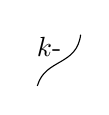
\begin{tikzpicture}[x=1cm,y=1cm,baseline=(n.base)]\node (n) at (0,0) {$k$-};\draw (-.15,-.5) .. controls (-.05,-.15) and (.35,-.25) .. (.4,.15);\end{tikzpicture}}schéma quasi-affine.

(iv) On peut faire opérer $G$ fidèlement sur un vectoriel sur $k$ (pas nécessairement de dimension finie).

(v) \deleted{(si $G$ est de type fini sur $k$),} $G$ est isomorphe à un sous-groupe fermé d'un groupe $\mathrm{Gl}(n)_k$ .

\uline{Démonstration}. On a (i)$\handwritten{\Rightarrow}$(ii) trivialement, et (ii)$\handwritten{\Rightarrow}$(iii), car $G$ opère fidèlement sur lui-même par translations à gauche. On a (iii)$\handwritten{\Rightarrow}$(iv) car si $G$ opère \deleted{fidèlement sur $X$ quasi-affine sur $k$, alors il opère fidèlement sur l'enveloppe affine $X'=\operatorname{Spec}(\handwritten{\Gamma}($}\inserted{sur $X$ quasi-compact et quasi-séparé sur $k$, il opère aussi} sur le vectoriel $\handwritten{\Gamma}(X,\underline{O}_X)$, grâce au fait que la formation de $f_{\handwritten{*}}(\underline{O}_X)$ ($f:X\handwritten{\to}\operatorname{Spec}k$ le morphisme structural) commute à tout changement de base $S\handwritten{\to}\operatorname{Spec}k$ (EGA IV 1.7.12); donc il opère sur l'enveloppe affine $X'=\operatorname{Spec}(\handwritten{\Gamma}(X,\underline{O}_X))$, et le morphisme canonique $X\handwritten{\to}X'$ est évidemment compatible avec l'action de $G$; ceci dit, si $X$ est quasi-affine i.e. $X\handwritten{\to}X'$ est une immersion ouverte, et si $G$ opère fidèlement sur $X$, il opère fidèlement sur $X'$, ou ce qui revient au même, sur le vectoriel $V=\handwritten{\Gamma}(X,\underline{O}_X)$, ce qui prouve l'implication (iii)$\handwritten{\Rightarrow}$(iv).

\handwritten{S}upposons maintenant \deleted{que $G$ est de type fini, et}\inserted{\handwritten{(iv), i.e.}} que $G$ opère fidèlement sur le vectoriel $V$. Alors\handwritten{,}en vertu de 11.10\handwritten{,}$V$ est limite inductive de sous-es\handwritten{p}aces vectoriels $V_i$ de di\handwritten{m}ension finie, stables sous l'action de $G$. Si $K_i$ est le noyau de l'action induite de $G$ sur $V_i$ , i.e. de $G\handwritten{\to}\underline{\operatorname{Aut}}_{\inserted{\handwritten{V_i}}}\deleted{\unsure{(V_i)}}$, alors $K_i$ est un sous-schéma fermé de $G$, et l'hypothèse que $G$ opère fidèlement s'exprime aussitôt par le fait que \deleted{$K_{\unsure{1|i|l}}=e$ (grou} l'intersection des $K_i$ est le sous-groupe unité de $G$. Comme $G$ est noethé%
% archive sheet number: 48
